\chapter{Tutorial}\label{chap:tutorial}
This chapter explains how to start \Pink and how to use it.

\section{Starting \Pink and related software}


\section{Examples}

We will show a lot of Python code:

Testing Listings:
\lstinputlisting{python/tut/hello.py}

Testing fancyvrb
\lstset{language=Python}

\mypylist{prog1}
\VerbatimInput[label=\fbox{\textbf{Program \ref{prog1}:} hello in Python}]{"python/tut/hello.py"}


Some code and its output

\mypylist{prog2}
\VerbatimInput[label=\fbox{\textbf{Program \ref{prog2}:} A plotting example}]{"python/test/plottest01.py"}

%% some embedded python
\begin{figure}
\centering
\begin{python}
import sys
sys.path.append('python/test')
import matplotlib
import plottest01
matplotlib.pyplot.savefig('dynamic/multiaxis.pdf')
print r'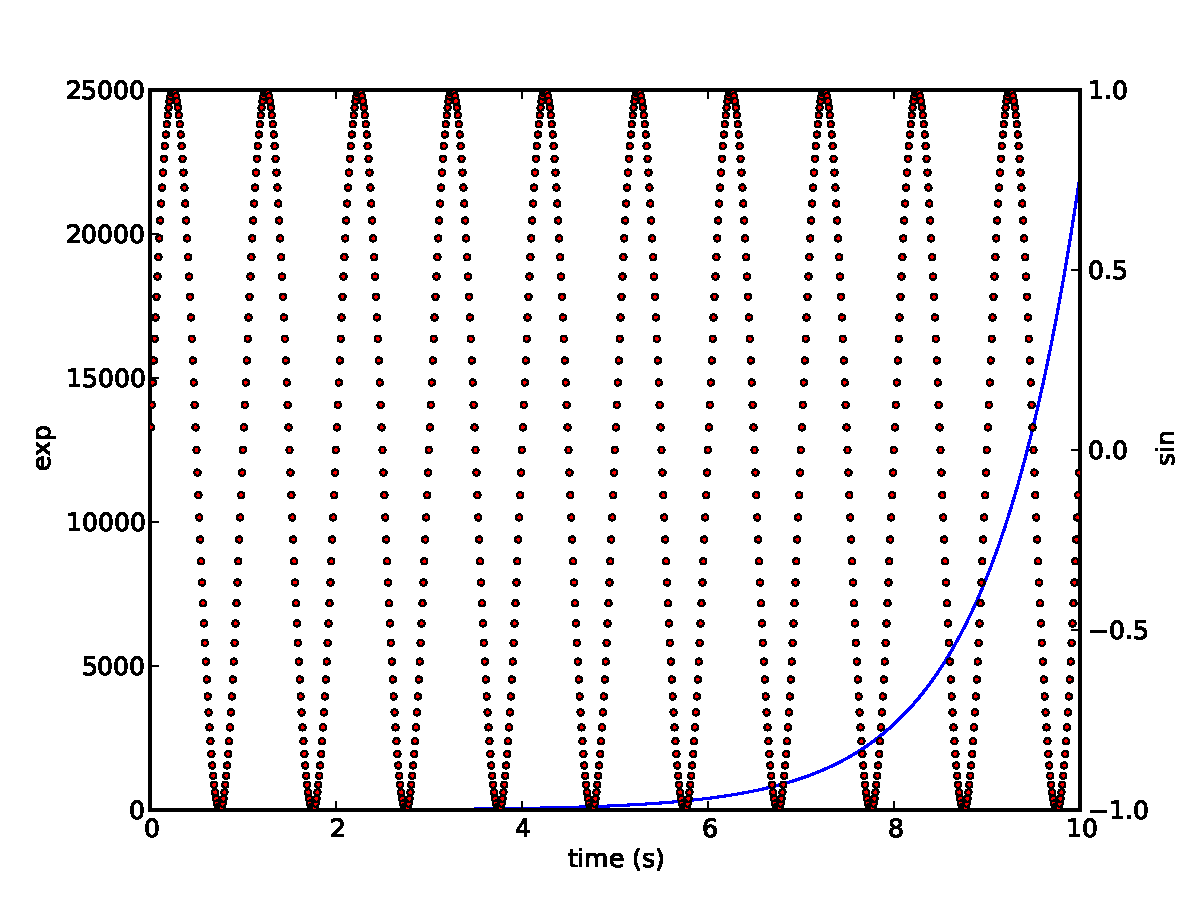
\includegraphics[width=0.5\textwidth]{dynamic/multiaxis.pdf}'
\end{python}
\caption{The functions $\sin$ and $\exp$ together from program~\ref{prog2}.}
\end{figure}


\subsection{Binary image processing}

\subsection{Grey-level segmentation}

\subsection{Discrete geometry}

\subsection{3D image processing}

\section{\Pink and other image-related software}

\subsection{\Pink and numpy}

\subsection{\Pink and scikit}

\subsection{\Pink and VTK}

\subsection{\Pink and ITK}

\section{Exercises}

